\section{Funktionen}
%	\begin{table}[h]
%		\centering
%		\resizebox{\textwidth}{!}{%
%			\begin{tabularx}{1\textwidth}{p{0.25\textwidth}ll}
%				\multicolumn{3}{l}{Sprungfunktion, Schrittfunktion, unit step} \\
%				\includegraphics[width=\textwidth]{./bilder/sprungF.png}      & x      & x      \\ \hline
%				\multicolumn{3}{l}{step} \\
%				&        &        \\ 
%			\end{tabularx}%
%		}
%	\end{table}
	
	\subsection{Impulsfunktion - dirac delta function}
		\begin{minipage}{0.2\textwidth}
			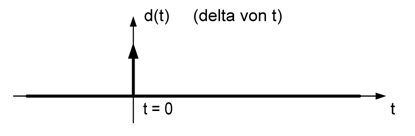
\includegraphics[width=\textwidth]{./bilder/funktionen/diracimpulse.png}
		\end{minipage}
		\qquad
		\begin{minipage}{0.45\textwidth}
			$\delta (t)=\begin{cases} 0 & t\ne 0\\\infty & t=0\end{cases} \qquad
			\text{und} \qquad \int\limits_{-\infty}^\infty \delta(t) \, \mathrm dt = 1 $\\
		\end{minipage}
		\qquad
		\begin{minipage}{0.25\textwidth}						
				$\int\limits_{-\infty}^{\infty}\delta(t-t_0)f(t)dt=f(t_0)$\\
	$\int\limits_{-\infty}^{\infty}\delta(at)\cdot f(t) dt = \frac{1}{|a|} \cdot f(0)$\\
	$s(t) \cdot \delta(t-t_0) = s(t_0)\cdot \delta(t-t_0)$\\
	Fouriertransformierte von $\delta(t)$:\\
	$\delta(t) \; \laplace \; 1(\omega)$ \hspace{0.5cm}
	$\delta(t-t_0) \; \laplace \; e^{-j\omega t_0}$ \hspace{0.5cm}
	$1(t) \; \laplace \; 2\pi \delta(\omega)$
		\end{minipage}
	
	\subsubsection{d-Funktion}
		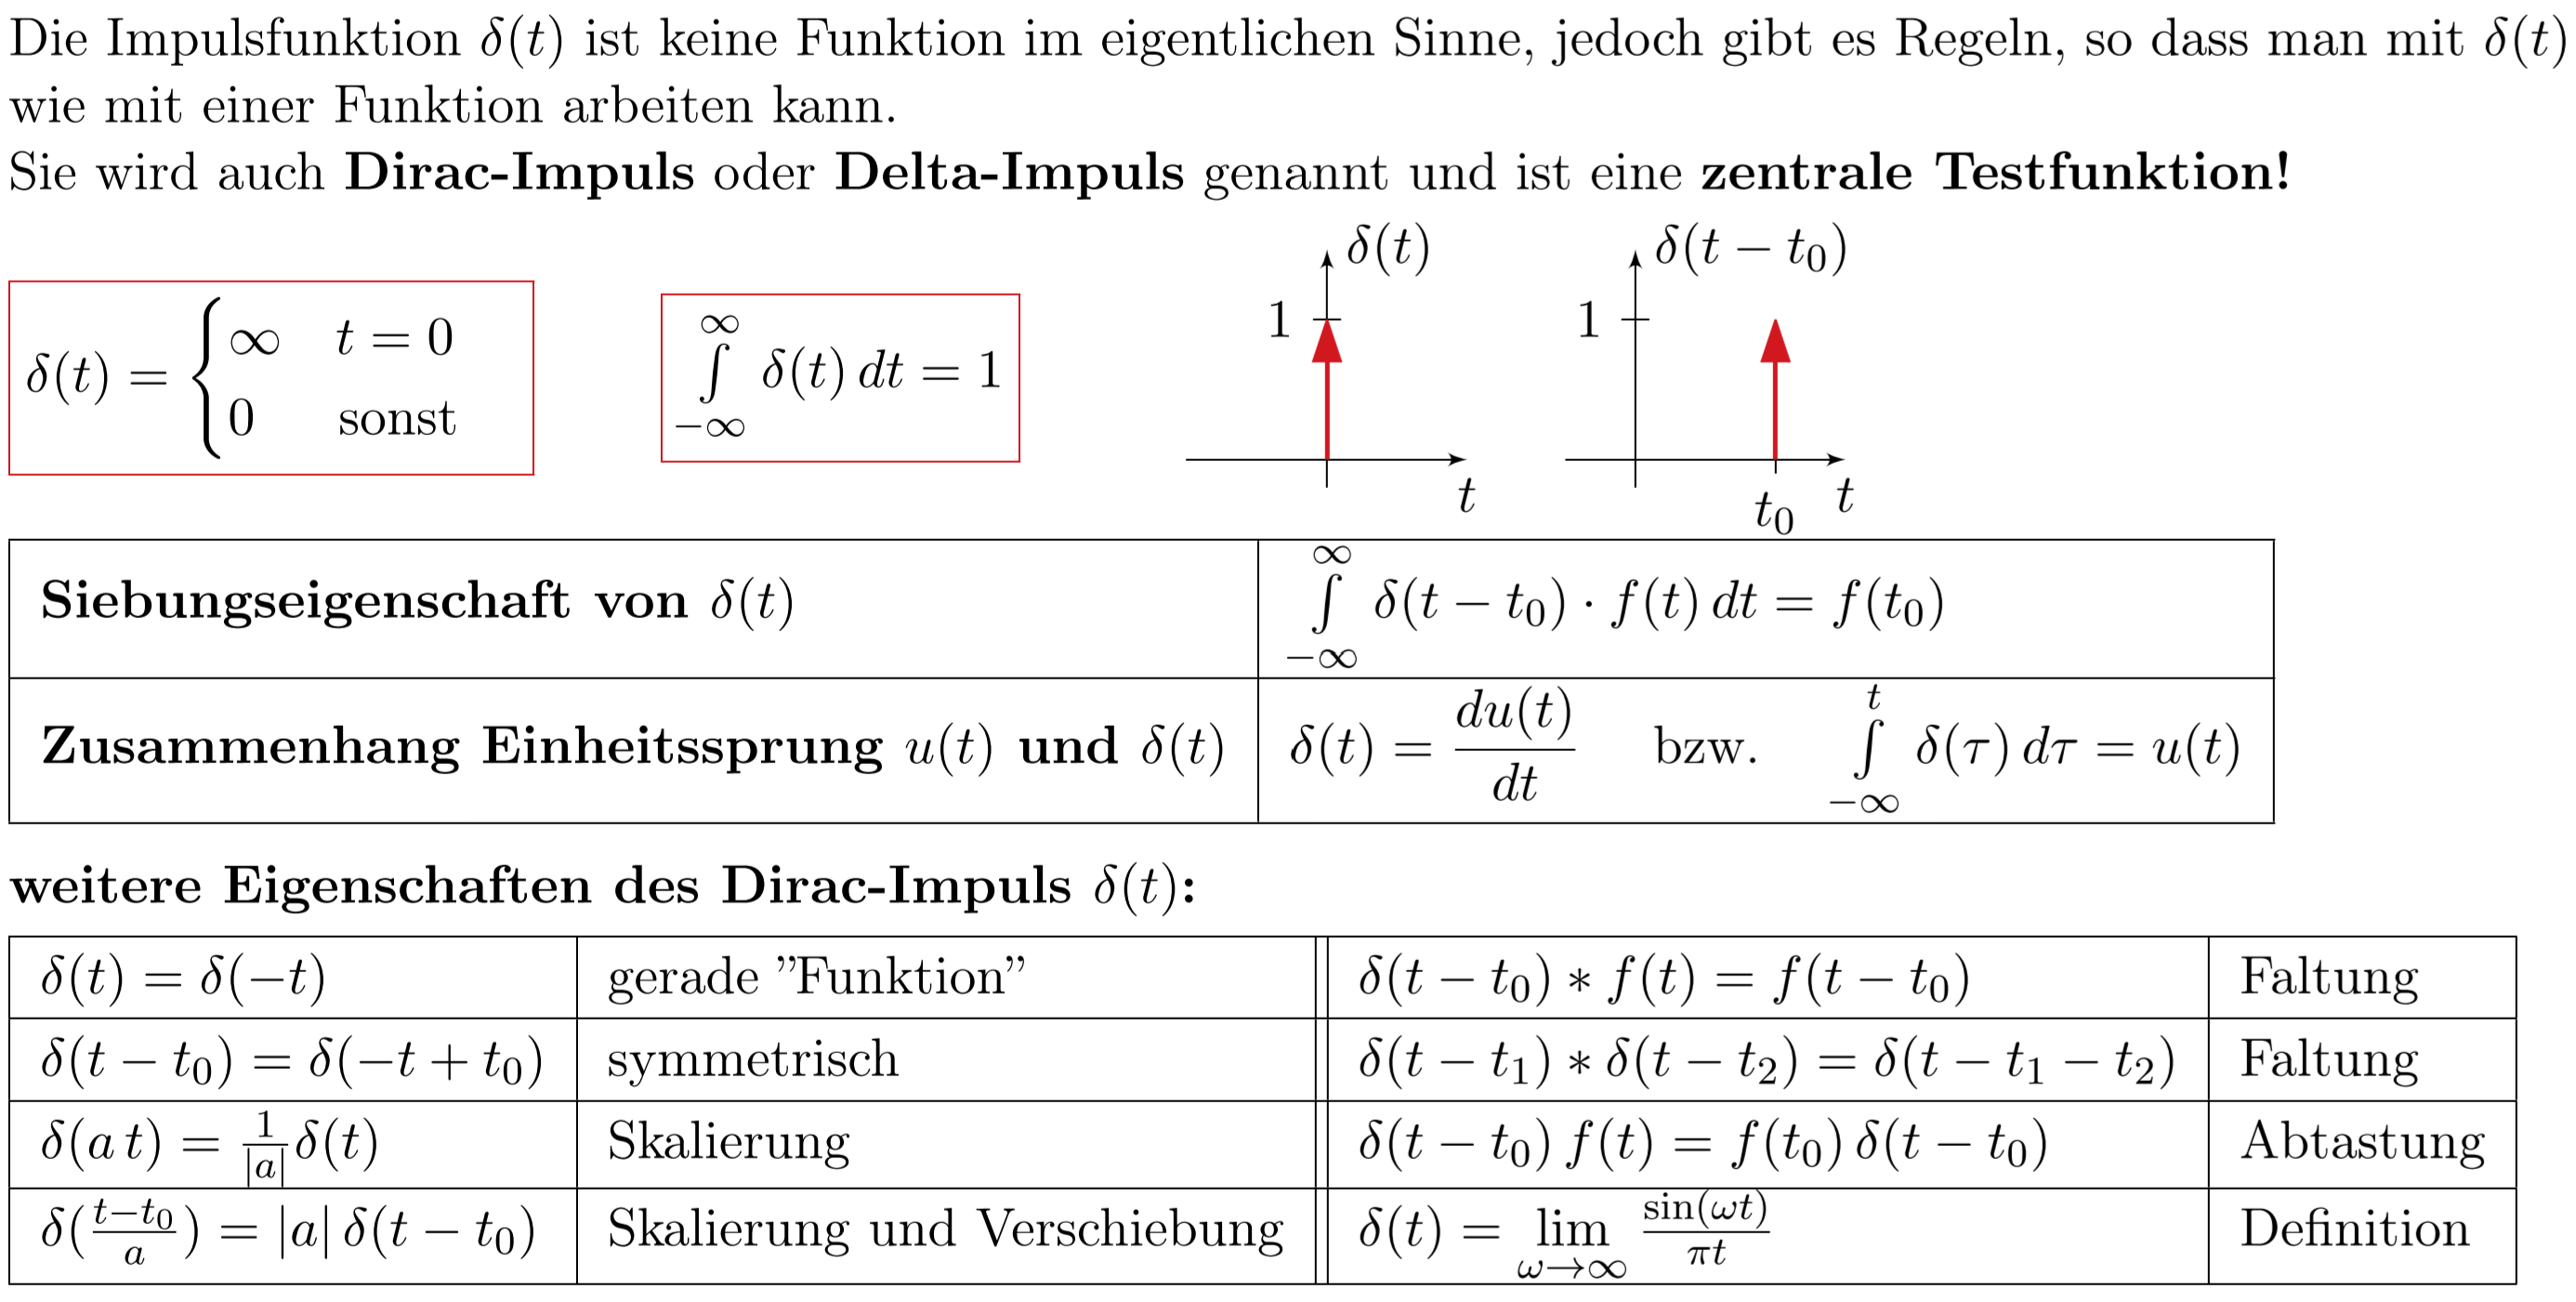
\includegraphics[width=0.8\textwidth]{./bilder/funktionen/impulsF.png}


	\subsection{Schrittfunktion - unit step}
		\begin{minipage}{0.2\textwidth}
			\includegraphics[width=\textwidth]{./bilder/funktionen/sprungF.png}
		\end{minipage}
		\qquad
		\begin{minipage}{0.45\textwidth}
			$u(t) = \sigma(t) =	\begin{cases}
			0 & \text{f\"ur } t < 0 \\
			\frac{1}{2} \text{(praxis)}  \text{ oder undef. (math.)} & \text{f\"ur } t = 0 \\
			1 & \text{f\"ur } t > 0
			\end{cases}$
		\end{minipage}
		\qquad
		\begin{minipage}{0.25\textwidth}						
			$\sigma(t) \; \laplace \; \frac{1}{j\omega} + \pi\delta(\omega) = \Sigma(\omega)$ \\
			\\
			$\frac{du(t)}{dt}=\delta(t)$\\
		\end{minipage}
	
	\subsection{Signumfunktion}
		\begin{minipage}{0.2\textwidth}
			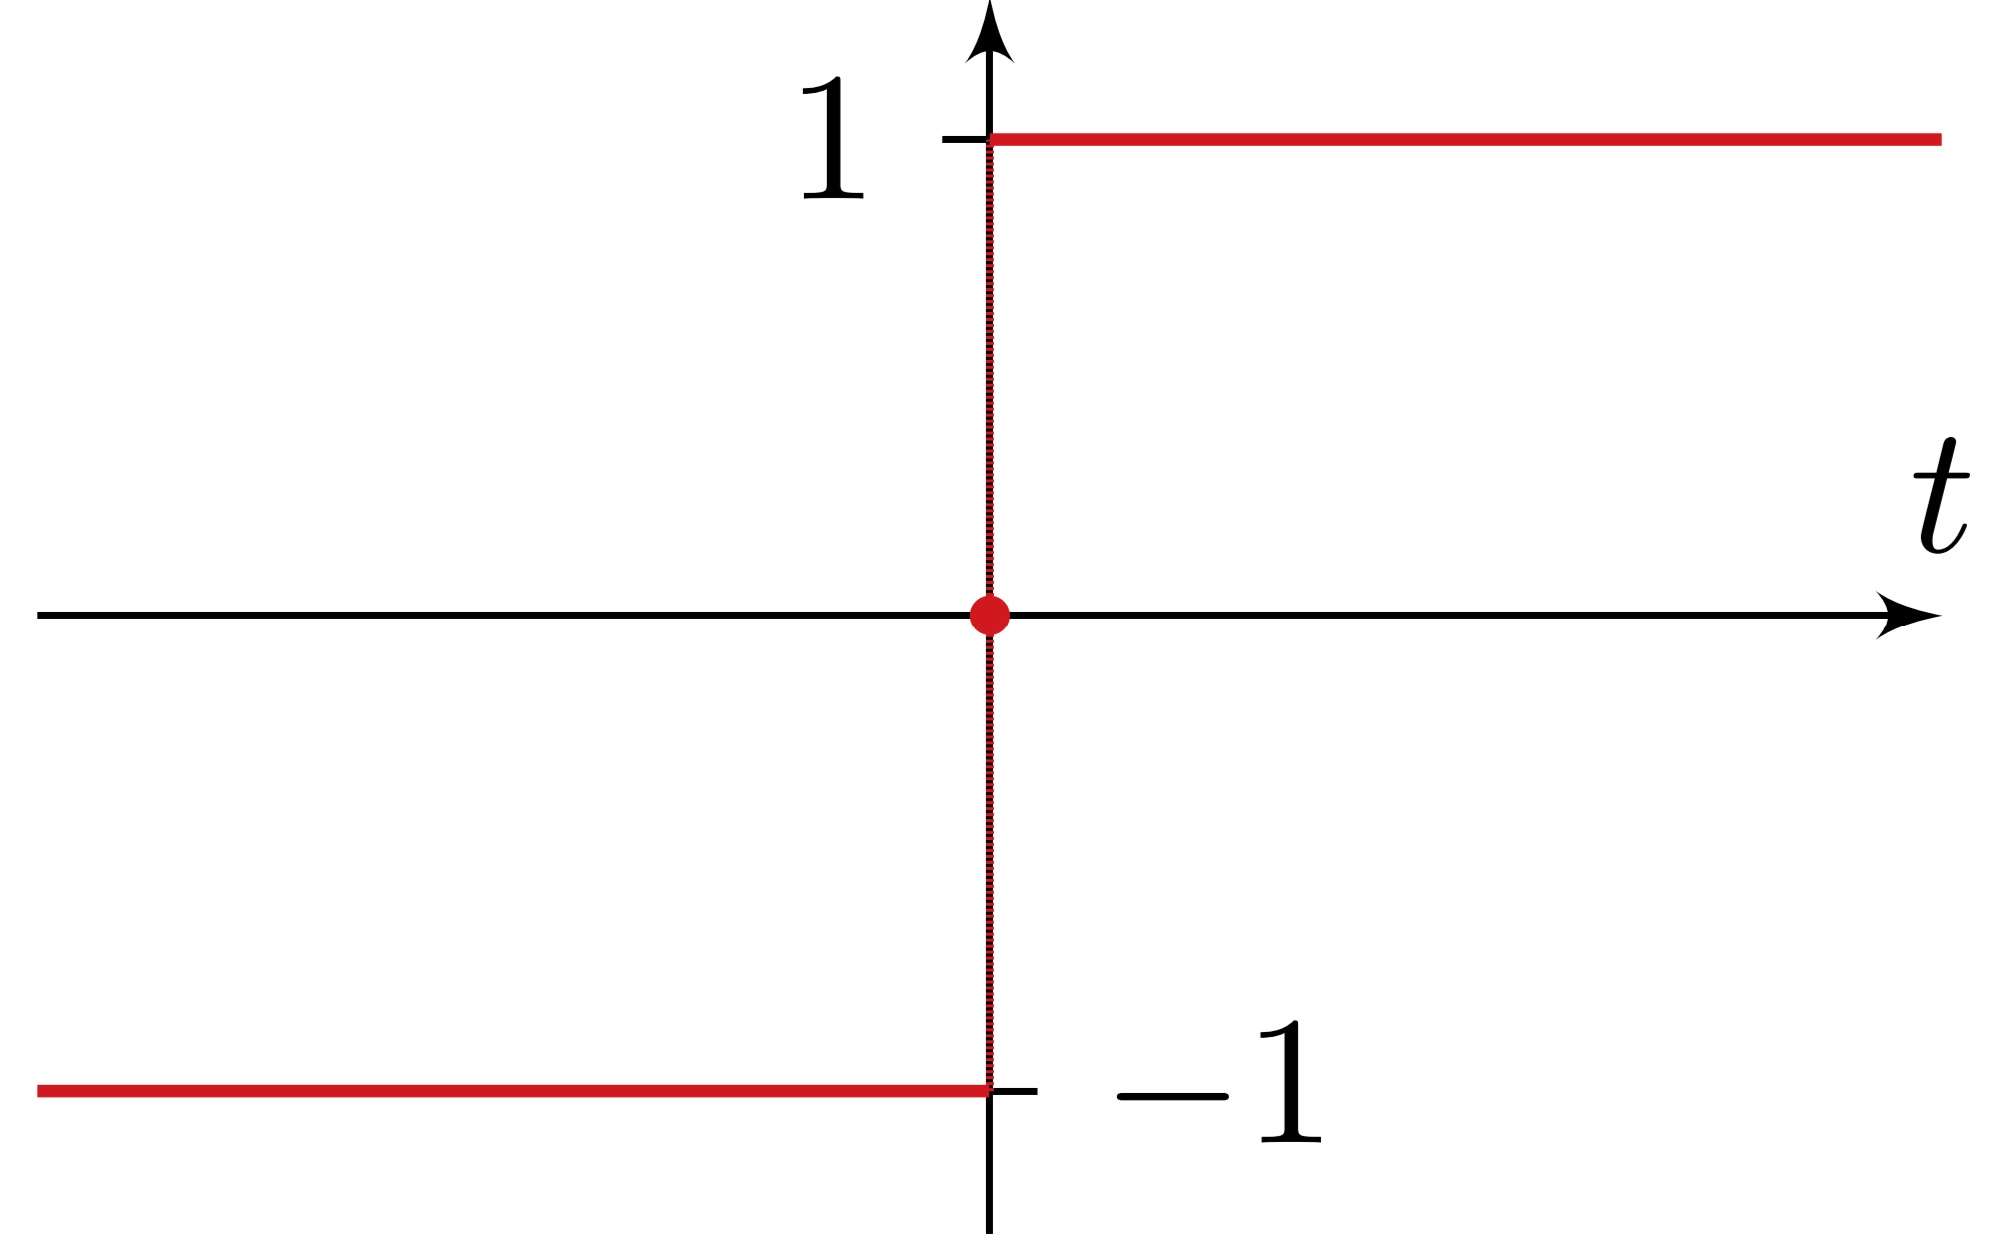
\includegraphics[width=\textwidth]{./bilder/funktionen/signF.png}
		\end{minipage}
		\qquad
		\begin{minipage}{0.45\textwidth}
			$sgn(t) = \begin{cases} 1 & \text{falls }t > 0 \\ -1 & \text{falls }t < 0 \end{cases}$
		\end{minipage}
		\qquad
		\begin{minipage}{0.25\textwidth}						
			$sgn(t) \; \laplace \; \frac{2}{j\omega}$\\
			\\
			$\frac{1}{\pi t} \; \laplace \; -j sgn(\omega)$\\
		\end{minipage}		

		
	\subsection{Rechteckimpuls}
		\begin{minipage}{0.2\textwidth}
			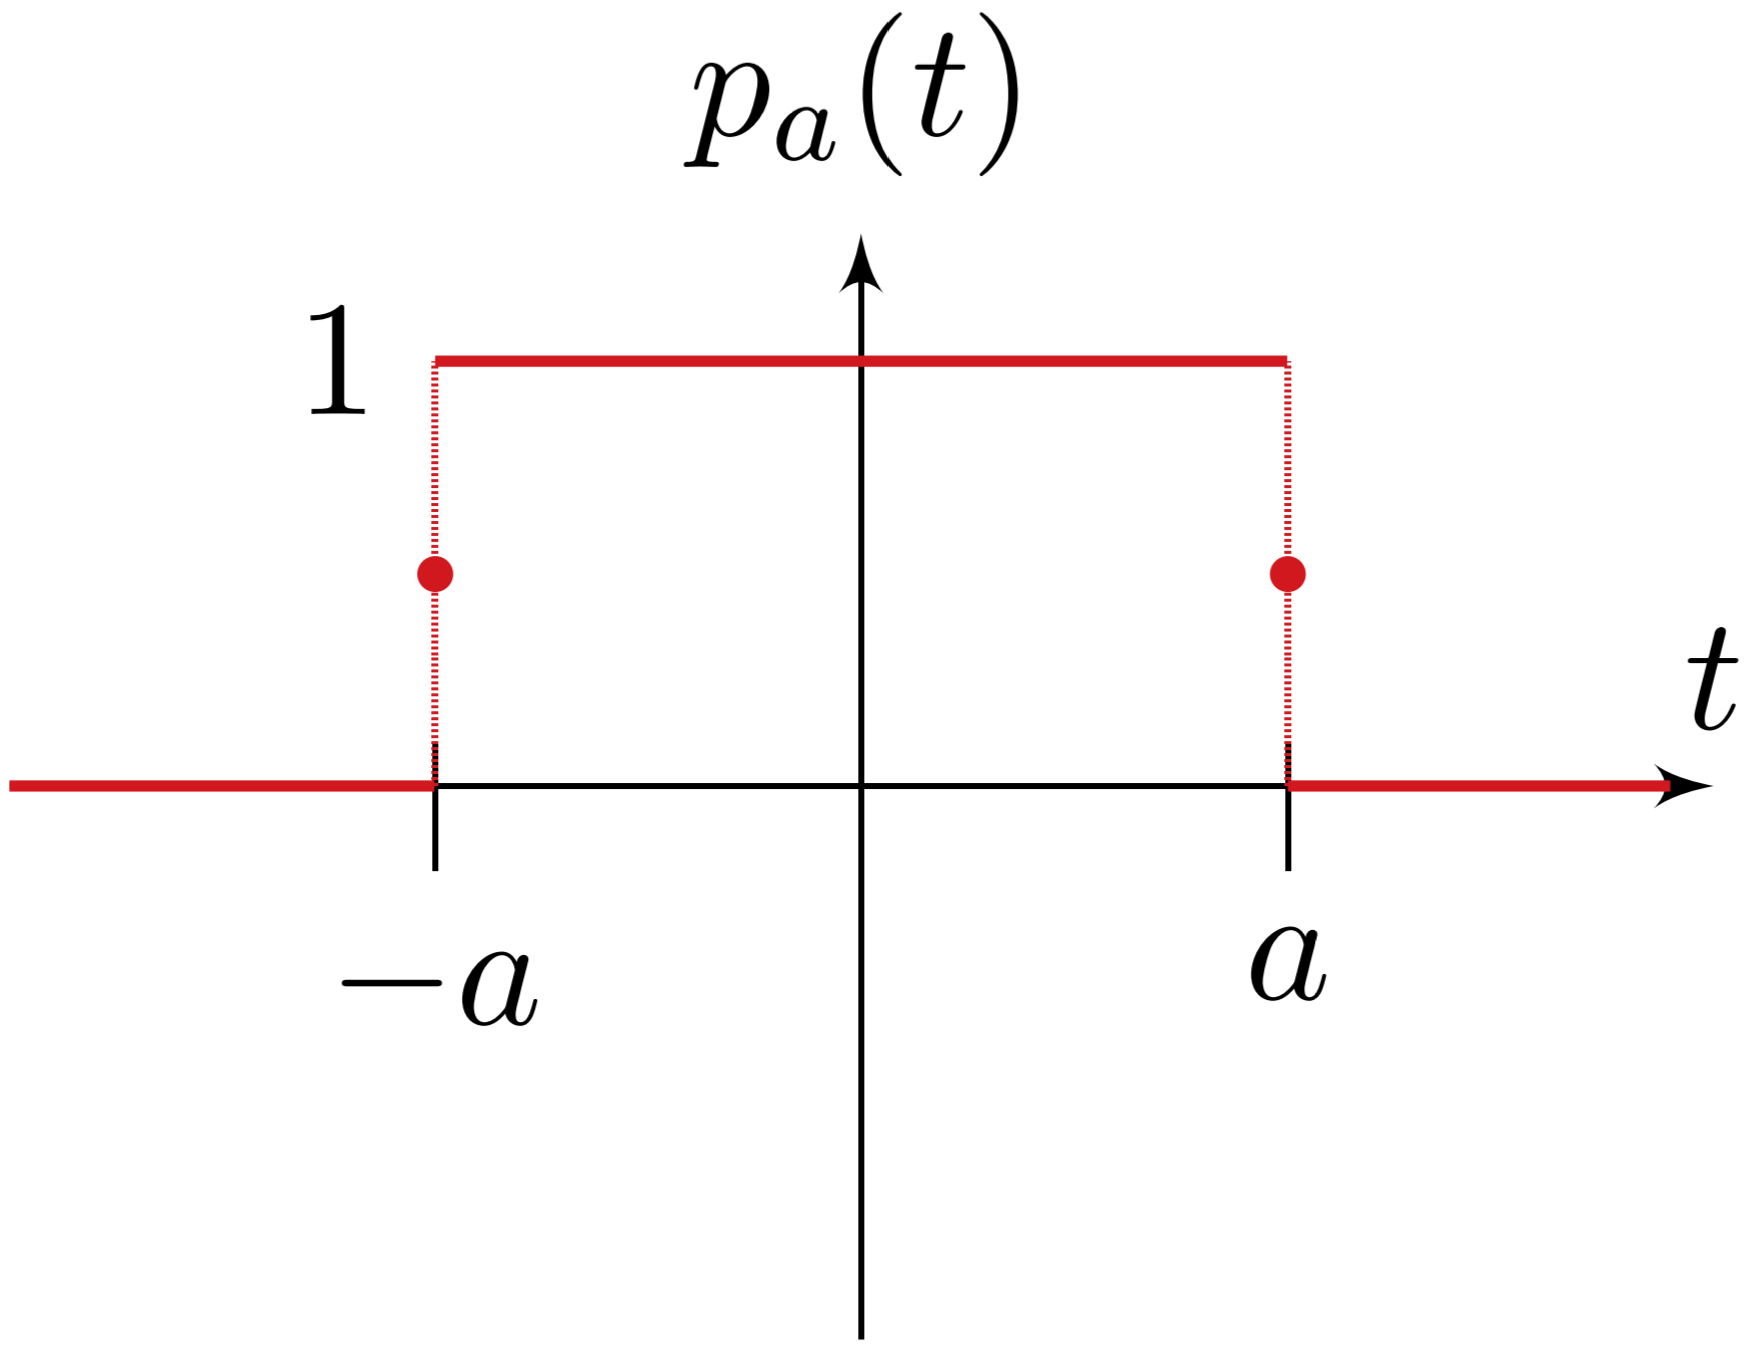
\includegraphics[width=\textwidth]{./bilder/funktionen/rechteckF.png}
		\end{minipage}
		\qquad
		\begin{minipage}{0.45\textwidth}
			$p_{a}(t)=\begin{cases}{1 & |t|<a \\ \frac{1}{2} & |t|=a \\ 0 & |t|>a}\end{cases}$
		\end{minipage}
		\qquad
		\begin{minipage}{0.25\textwidth}						
			$sgn(t) \; \laplace \; \frac{2}{j\omega}$\\
			\\
			$\frac{1}{\pi t} \; \laplace \; -j sgn(\omega)$\\
		\end{minipage}
			\begin{tabular}{p{9cm} p{9cm}}
				$r_T(t) \; \laplace \; \frac{2}{\omega} \cdot \sin(\omega T) \Rightarrow$ sinc-Funktion &
				$\int\limits_{-\infty}^{\infty} \frac{\sin(a \omega)}{\omega} d\omega = 
				\begin{cases} \pi & \text{falls }a > 0 \\ -\pi & \text{falls }a < 0 \end{cases}$
			\end{tabular}
	
	\subsection{Funktionen manipulieren}
		\includegraphics[width=\textwidth]{./bilder/SignalManip.png}